\documentclass{article}

% Packages
\usepackage{lipsum} % For generating dummy text
\usepackage{graphicx} % For including images
\usepackage{subcaption} % For subfigures
%\usepackage{cite} % For citations
\usepackage{hyperref} % For hyperlinks
\usepackage{float} % For positioning figures

% Title page information
\title{InfiniTerra: An Infinite Terrain Generation System}
\author{Mirto Randellini}
\date{\today}

\begin{document}

% Title page
\maketitle

% Table of contents
\tableofcontents

%enforce new page
\newpage

% Abstract
\begin{abstract}
	Infinite terrains are a crucial component in video games and real-time applications, providing
	players with vast, boundaryless worlds to explore. This report presents the design and 
	implementation of InfiniTerra, an infinite terrain generation system. The report discusses the 
	theory behind terrain generation, the algorithms used, and the rendering techniques employed to 
	display the terrain. It also addresses the challenges faced in creating an infinite terrain 
	system and how they were overcome. By leveraging heightmap generation techniques based on ridged 
	Perlin noise and utilizing compute shaders for performance optimization, InfiniTerra achieves 
	efficient and visually appealing terrain generation. The report concludes with a discussion on 
	the benefits and potential applications of the InfiniTerra system.
\end{abstract}

% Introduction
\section{Introduction}
\label{ch:introduction}
% Why make an infinite terrain?
Infinite terrains are a common feature in video games and other real-time applications, like flight
simulators and virtual reality experiences. They allow for the creation of vast, open worlds that
players can explore without encountering any boundaries. This can enhance the sense of immersion
and freedom in a game, as players can travel in any direction without being constrained by the size
of the game world. In this report, we will discuss the design and implementation of an infinite
terrain generation system called InfiniTerra. We will cover the theory behind terrain generation,
the algorithms used to generate the terrain, and the rendering techniques used to display the
terrain to the player. We will also discuss the challenges of creating an infinite terrain system
and how they were overcome in the development of InfiniTerra.

\begin{figure}[H]
	\centering
	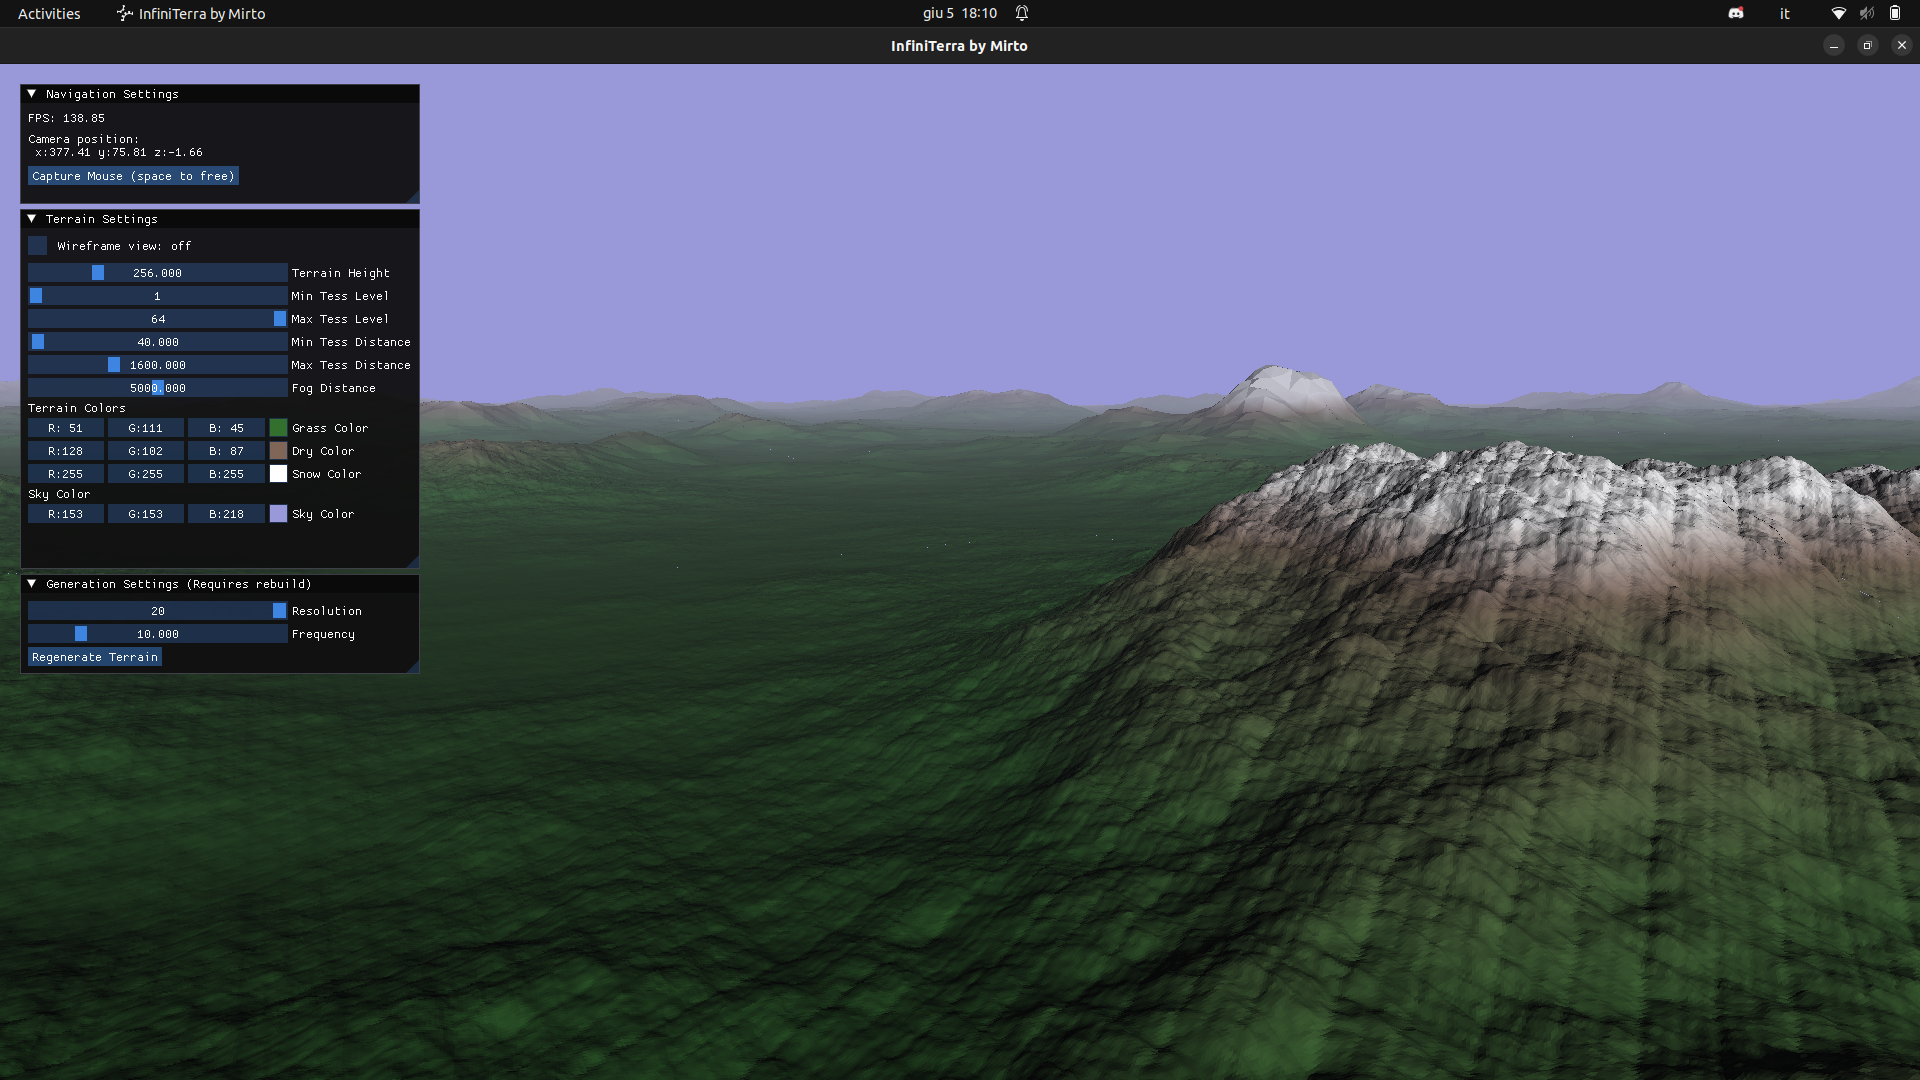
\includegraphics[width=0.75\textwidth]{img/infiniterra.png}
	\caption{InfiniTerra running on a modern GPU.}
	\label{fig:infiniterra}
\end{figure}

% Relevant existing work in games
\section{Background}
Before diving into the details of the system, it is useful to mention some of the existing work in
the field of terrain generation. The earliest use of procedural generation in games can be traced
back to the 1980s, with games like \textit{Hack} and \textit{Rogue}. These games used procedural
generation to create dungeons and levels that were different each time the player played the game
and they spawned a whole genre of games known as roguelikes.

\begin{figure}[H]
	\centering
	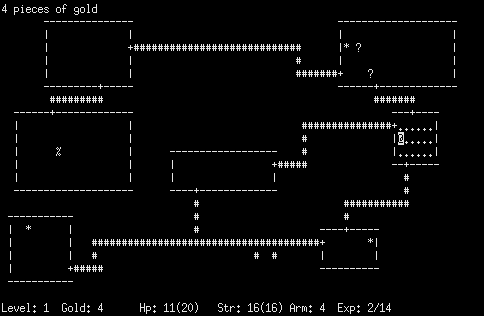
\includegraphics[width=0.75\textwidth]{img/rogue.png}
	\caption{A procedurally generated dungeon map in the videogame Rogue.}
	\label{fig:nethack}
\end{figure}

Moving forward to 1996, the game \textit{Elder Scrolls II: Daggerfall} featured a procedurally
generated world with a size of 161,600 square kilometers (approximately the size of England), which
was the largest game world ever created at the time, and it is still one of the largest game worlds
ever created. To be precise the wilderness between locations is based on a rudimentary heightmap,
one pixel of which covers 800 in-game metres. Smaller details are randomly generated, while actual
locations are pre-generated, and are consequently always the same.

\begin{figure}[H]
	\centering
	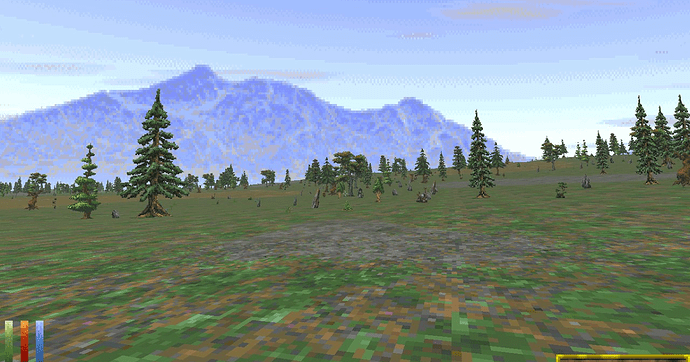
\includegraphics[width=0.75\textwidth]{img/daggerfall.png}
	\caption{The procedurally generated world map of the game Elder Scrolls II: Daggerfall.}
	\label{fig:daggerfall}
\end{figure}

Today one of the most famous examples of procedural generation in games is \textit{Minecraft}, a
game that features a procedurally generated world made up of blocks that players can mine and place
to create their own structures. The world in Minecraft is generated using Perlin noise, a type of
gradient noise that is commonly used in procedural generation to create natural-looking terrains.
The generation algorithm has then been improved over the years to include more complex features
like caves, villages, and biomes.

\begin{figure}[H]
	\centering
	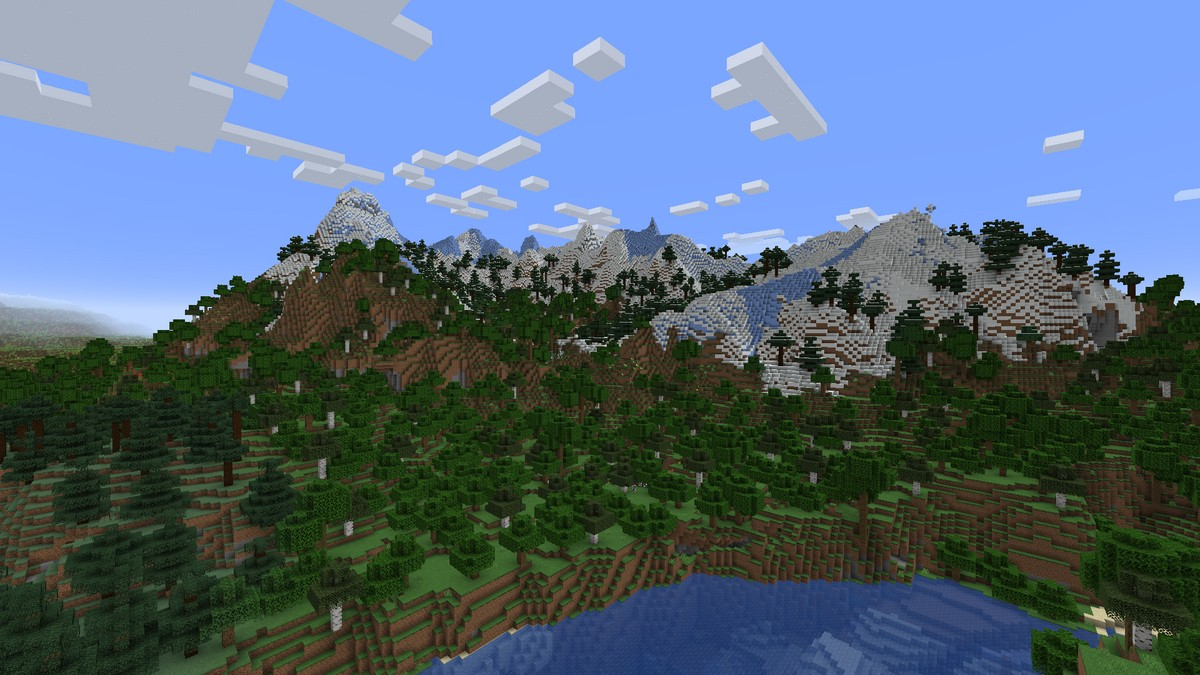
\includegraphics[width=0.75\textwidth]{img/minecraft.jpg}
	\caption{A procedurally generated world in the videogame Minecraft.}
	\label{fig:minecraft}
\end{figure}

% End introduction

\section{Generating the terrain}
\label{ch:generating-the-terrain}
% Heightmap generation
Commonly used techniques for terrain generation include heightmap generation, fractal terrain
generation, and procedural generation using noise functions. These techniques use mathematical
functions to generate terrain data that can be used to displace the vertices of a grid to create a
3D terrain. In InfiniTerra, we use a heightmap generation technique based on ridged Perlin noise to
create the terrain.
% Perlin noise
\subsection{Perlin Noise}
Perlin noise is a type of gradient noise developed by Ken Perlin in 1983. It is commonly used in
computer graphics to create natural-looking textures and terrains. We note that its first use was
in the movie Tron (1982) to create the light cycle effects.

\begin{figure}[H]
	\centering
	\begin{subfigure}[h]{0.35\textwidth}
		
\includegraphics[width=\textwidth]{img/perlin_noise.png}
		\caption{Perlin noise.}
		\label{fig:pnoise}
	\end{subfigure}
	\hfill
	\begin{subfigure}[h]{0.55\textwidth}
		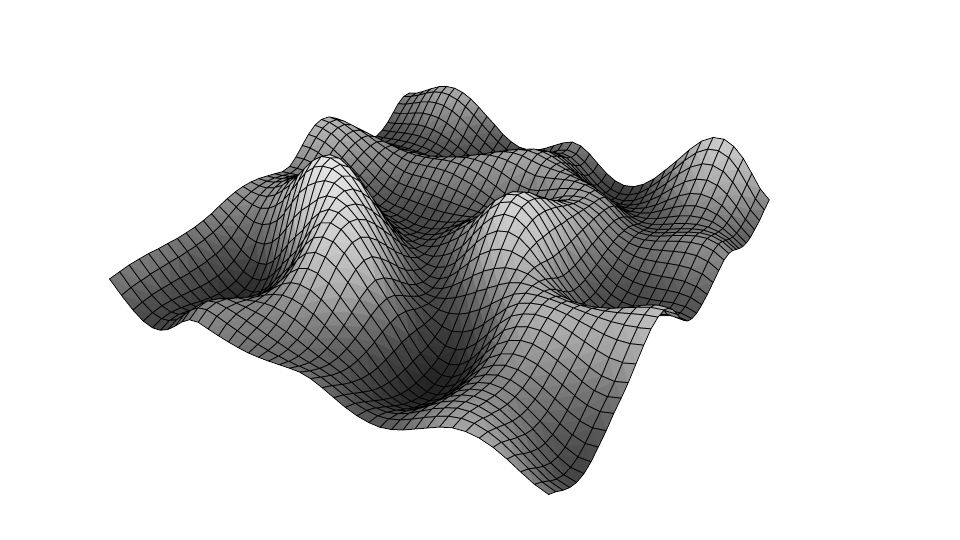
\includegraphics[width=\textwidth]{img/perlin_terrain.png}
		\caption{Perlin noise used to displace the vertices of a grid.}
		\label{fig:pterrain}
	\end{subfigure}
\end{figure}

Perlin noise is computed by generating a grid and for each point of the grid, a random gradient
vector. The value of the noise in each point is then computed by calculating the dot product
between the gradient vectors and the distance vectors from the point to the four corners of the
grid cell. The noise value is then interpolated to create a smooth transition between the points.

\begin{figure}[H]
	\centering
	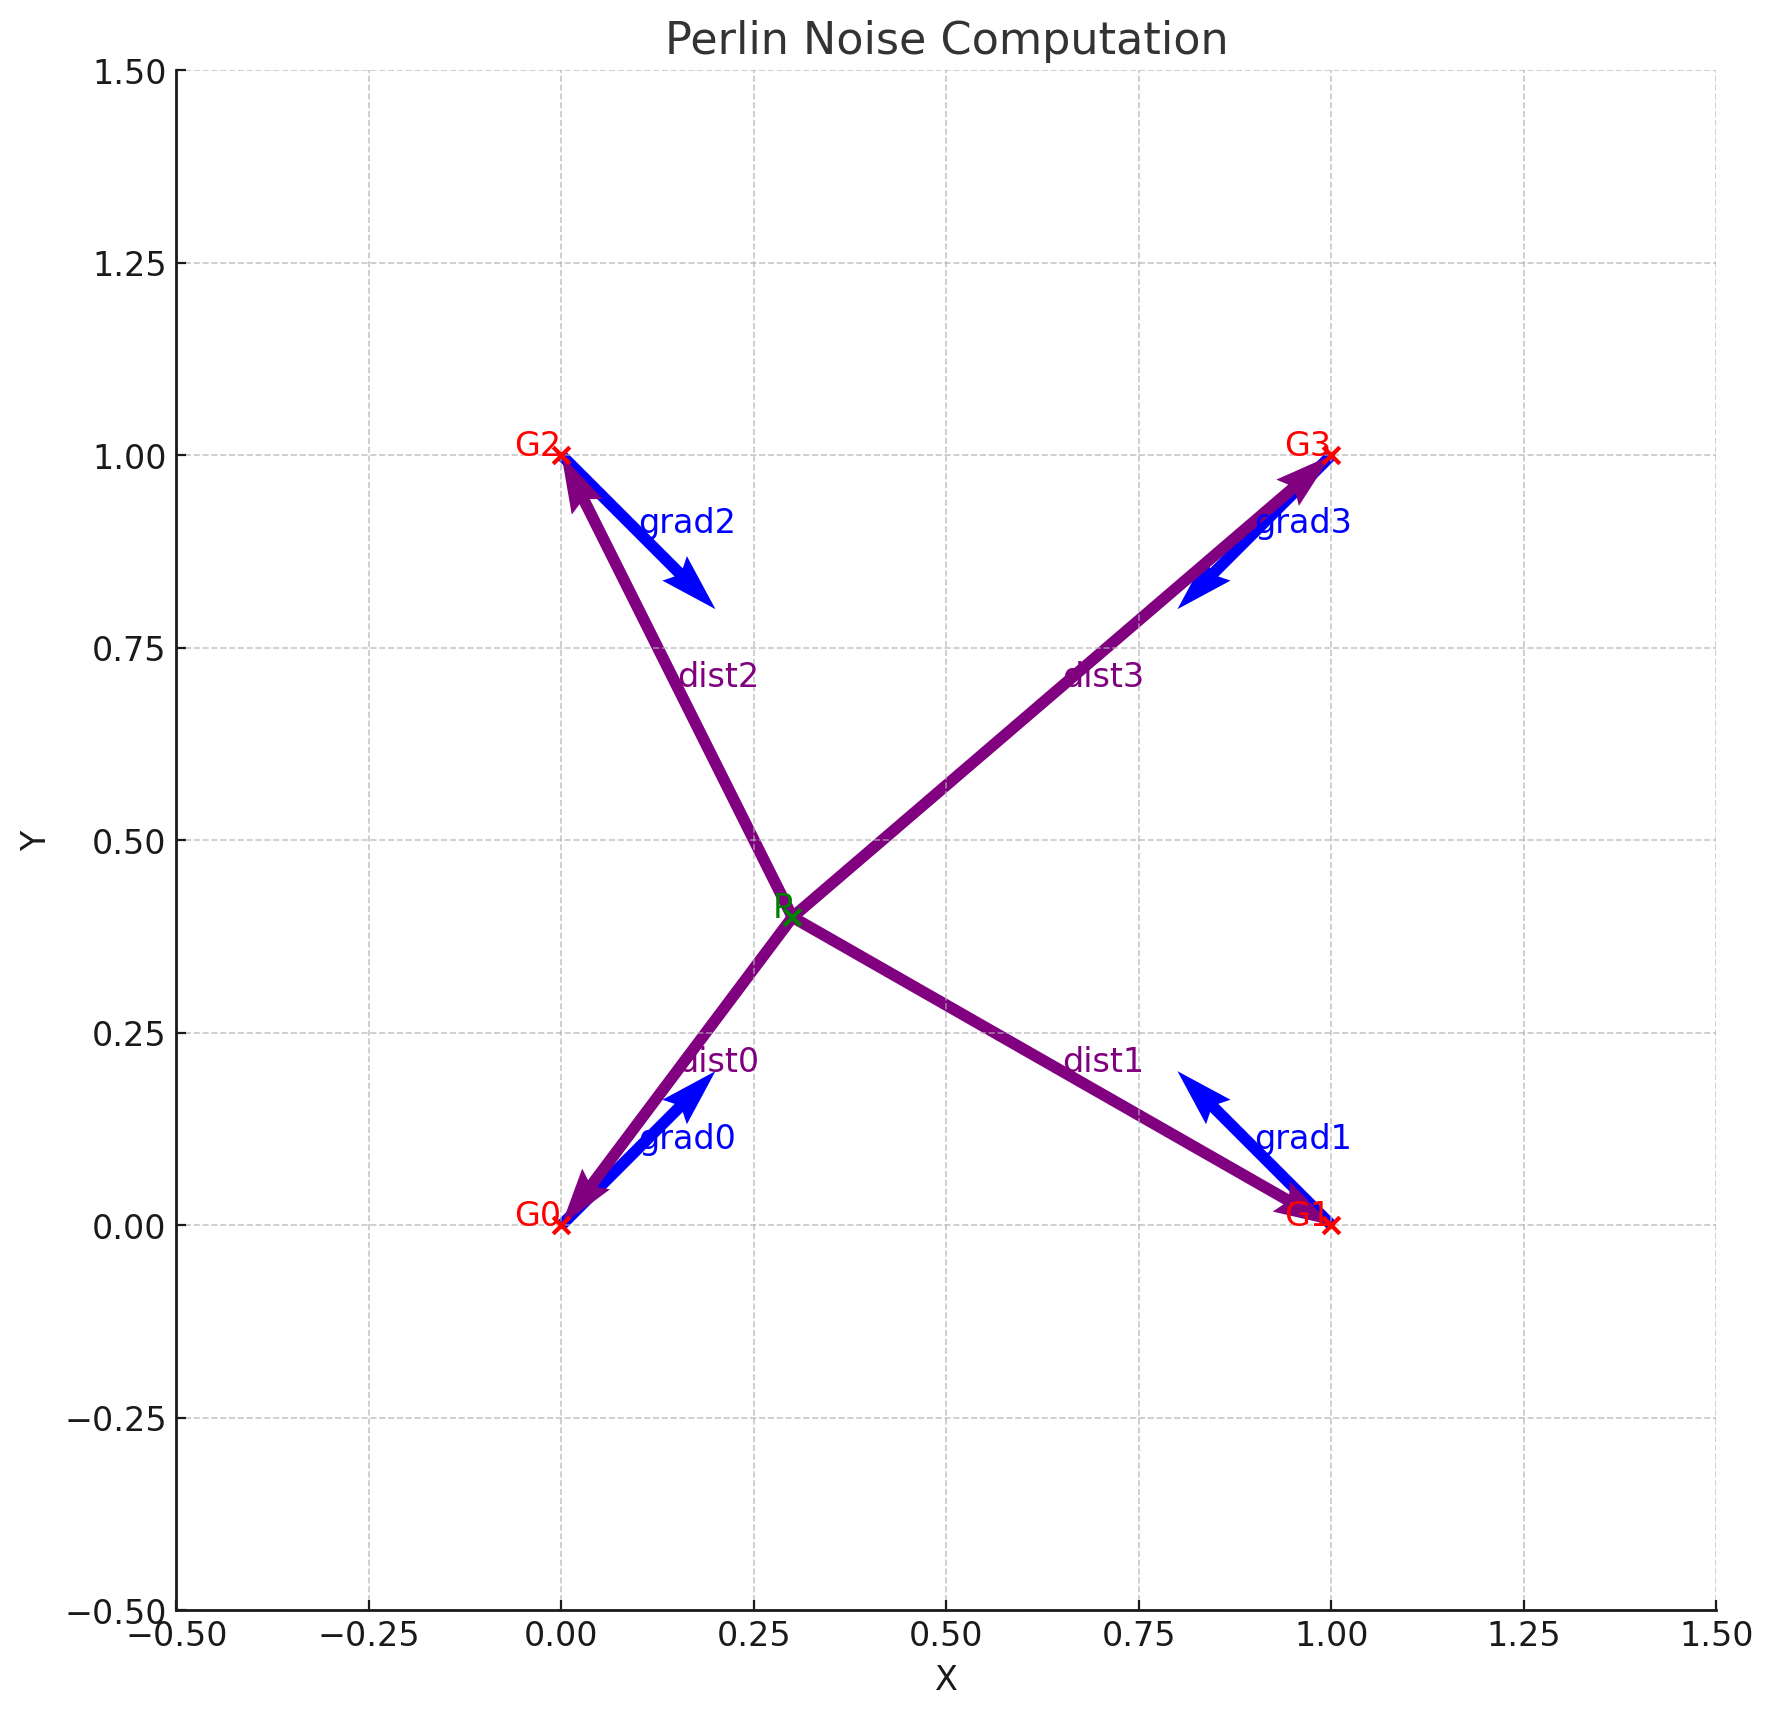
\includegraphics[width=0.55\textwidth]{img/perlin.png}
	\caption{The vectors involved in the computation of Perlin noise.}
	\label{fig:perlin_vectors}
\end{figure}

% Ridged Perlin noise?
In InfiniTerra, we use a variation of Perlin noise called ridged Perlin noise to create the terrain.
Ridged Perlin noise is a type of Perlin noise that has sharp peaks and valleys, which can be used to
create more realistic terrains. The ridged Perlin noise function is computed by taking the absolute
value of the Perlin noise function and subtracting it from 1.

$$ ridgedPerlin(x, y) = 1 - |perlin(x, y)| $$

\begin{figure}[H]
	\centering
	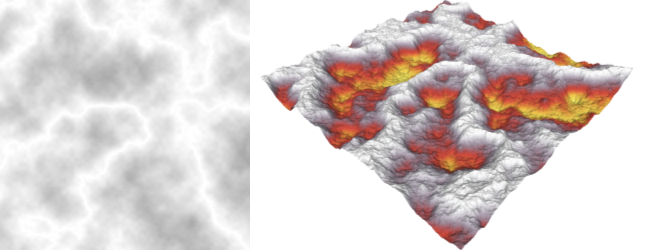
\includegraphics[width=0.75\textwidth]{img/ridged_perlin.png}
	\caption{Ridged Perlin noise.}
	\label{fig:rnoise}
\end{figure}

% CPU implementation
\subsubsection{CPU Implementation}
In the first version of the system, the heightmap generation was implemented on the CPU by using
the FastNoiseLite library. This allowed access to a wide variety of noise functions, such as
Perlin, Simplex, and Cellular noise, but was not performant enough for generating large terrains.
The generation of a 1024x1024 heightmap took around 5s on a modern CPU, which was too slow for
real-time applications.
% GPU implementation (compute shaders)
\subsubsection{GPU Implementation}
To improve performance, the heightmap generation was moved to the GPU by using compute shaders.
The function used to generate the terrain is the ridged Perlin noise function was taken from 
\textit{patriciogonzalesvivo}'s github repository. The compute shader generates the heightmap by
computing the ridged Perlin noise function for each point of the grid and writing the result to a
texture. The texture is then used to displace the vertices of the terrain.

\subsection{Compute shaders}
% Introduce the pipeline and shader stages
In modern graphics programming, the rendering pipeline is divided into several stages, each of
which is implemented using a different type of shader.

\begin{figure}[H]
	\centering
	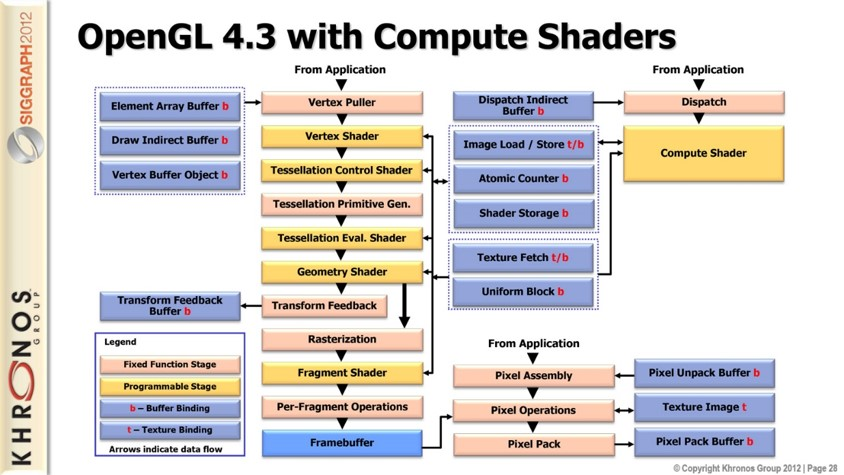
\includegraphics[width=0.75\textwidth]{img/compute_shaders.jpg}
	\caption{The graphics rendering pipeline.}
	\label{fig:pipeline}
\end{figure}

A Compute Shader is a type of shader stage that is primarily used for performing arbitrary 
computations. Although it has the capability to render, its main use is for tasks that are not 
directly associated with rendering triangles and pixels. It is utilized for executing 
general-purpose computing tasks on the GPU, such as physics simulations, image processing, and 
data processing. The compute shader runs in parallel using multiple threads, enabling it to 
compute much faster than the CPU. Compute shaders are not included in the standard rendering 
pipeline. Therefore, when a Drawing Command is executed, the compute shader linked to the current 
program or pipeline is not engaged. Instead, you must specifically dispatch a compute shader to run 
on the GPU. Compute shaders function in an abstract space known as a dispatch grid, a 3D grid of 
thread groups, referred to as \textit{work groups}. The system can compute these work groups in any 
sequence. For instance, given a work group set of (3, 1, 2), it could first execute group (0, 0, 0), 
then move to group (1, 0, 1), and then to (2, 0, 0), and so on. Therefore, your compute shader 
should not depend on the sequence in which individual groups are processed. A single work group is 
not equivalent to a single compute shader invocation; hence it is called a \textit{group}. A single 
work group can contain multiple compute shader invocations, the number of which is determined by 
the compute shader itself, not the call that executes it. This is referred to as the local size of 
the work group. Each thread group consists of multiple threads, which can interact using shared 
memory. This enables the compute shader to carry out complex computations that require thread 
synchronization. A compute shader does not have the same inputs and outputs as other shader stages, 
but it can read from and write to buffers and textures, enabling it to perform a broad range of 
computations.

\begin{figure}[H]
	\centering
	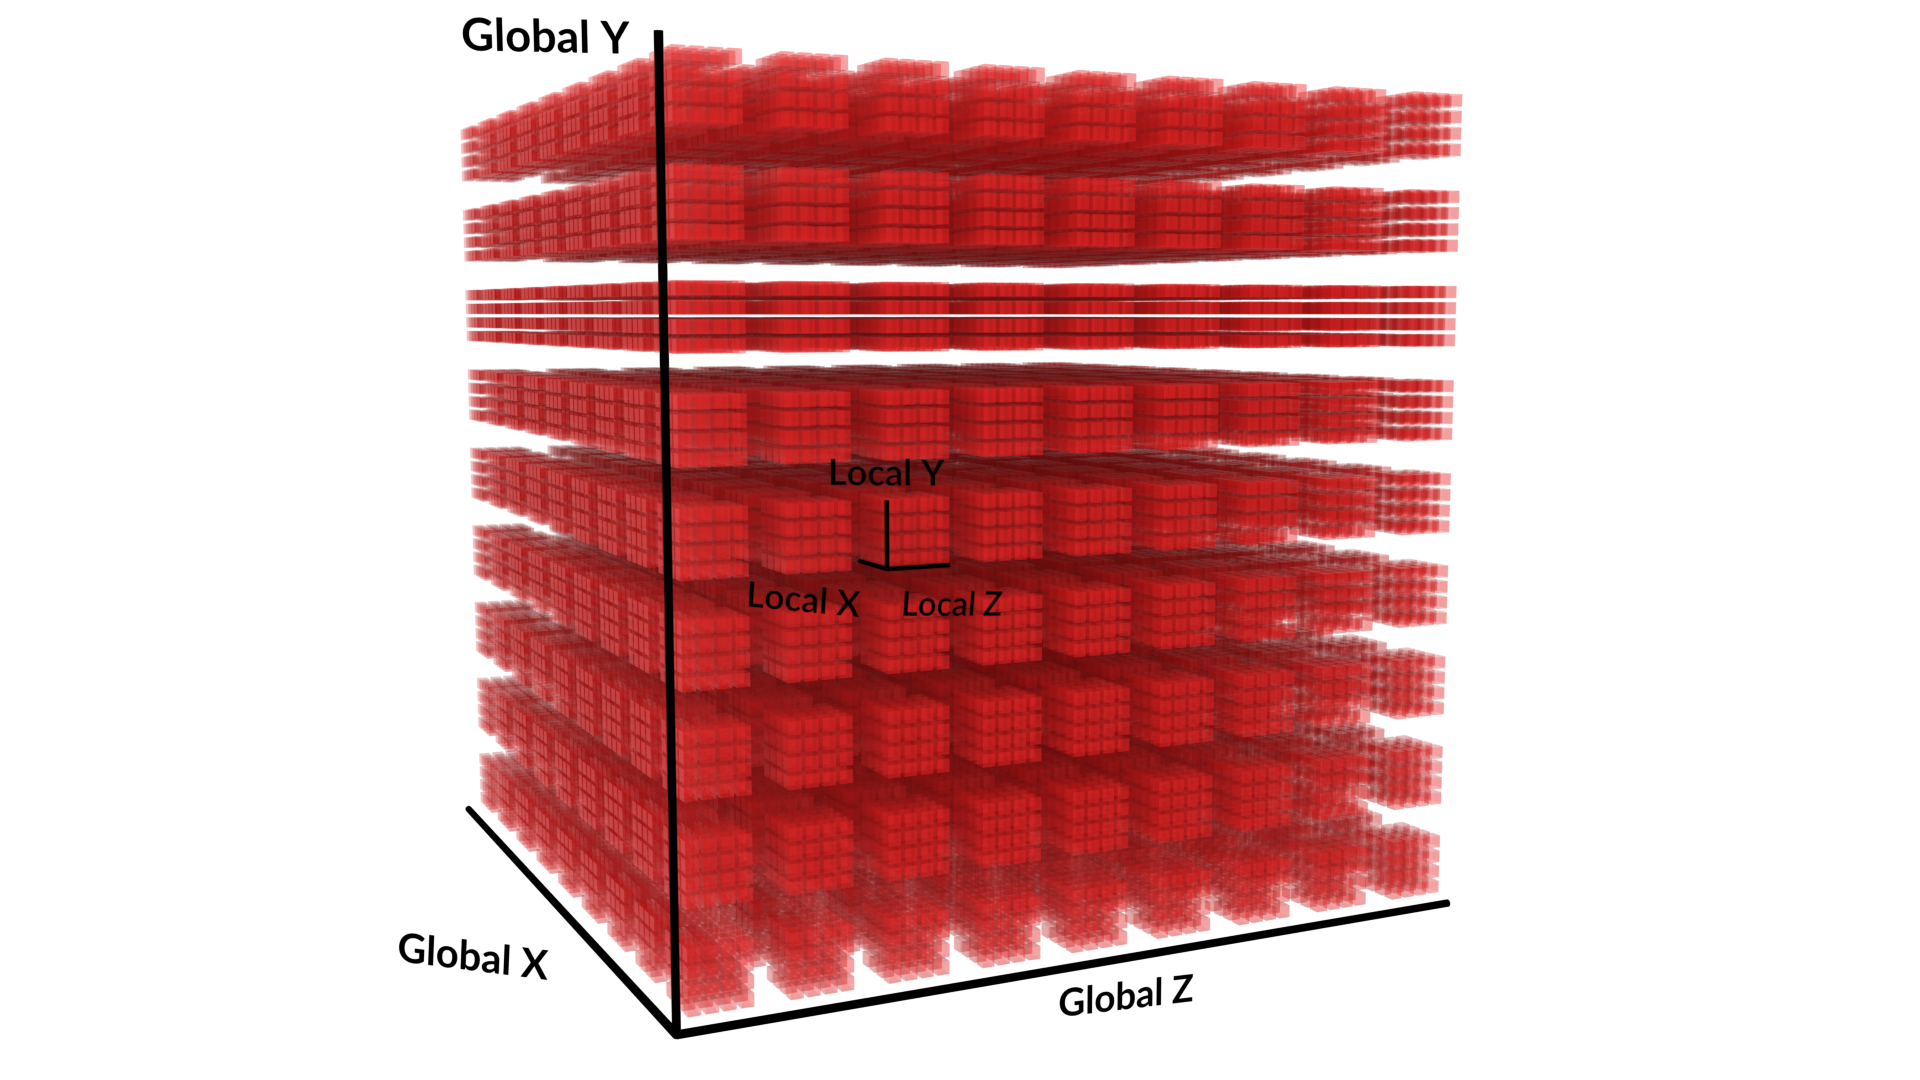
\includegraphics[width=0.75\textwidth]{img/work_groups.png}
	\caption{work groups split in their local space invocations, represented by the red cubes.}
	\label{fig:work_groups}
\end{figure}

\section{Rendering the terrain}
\label{ch:rendering-the-terrain}
% Base geometry (triangles) Phong Lighting
\subsection{Phong Lighting}

Phong lighting is a shading model developed by Bui Tuong Phong in 1975. It is a local illumination
model that approximates the way light interacts with a surface by using three components: ambient,
diffuse, and specular. The ambient component represents the light that is scattered in all
directions and is reflected equally by all surfaces. The diffuse component represents the light
that is scattered in all directions but is reflected more in the direction of the light source. The
specular component represents the light that is reflected in a specific direction, which is
determined by the angle between the light source and the viewer.

\begin{figure}[H]
	\centering
	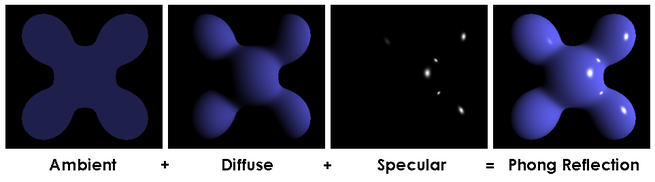
\includegraphics[width=0.75\textwidth]{img/phong.png}
	\caption{The components of Phong lighting.}
	\label{fig:phong}
\end{figure}

% Phong lighting implementation

\subsection{Implementation}
Phong lighting is computed using the following formula: $$ I = k_a \cdot I_a + k_d \cdot I_d \cdot
	(\hat{L} \cdot \hat{N}) + k_s \cdot I_s \cdot (\hat{R} \cdot \hat{V})^n $$ where:
\begin{itemize}
	\item $I$ is the intensity of the light at the surface point.
	\item $k_a$ is the ambient reflection coefficient.
	\item $I_a$ is the intensity of the ambient light.
	\item $k_d$ is the diffuse reflection coefficient.
	\item $I_d$ is the intensity of the diffuse light.
	\item $\hat{L}$ is the unit vector pointing from the surface point to the light source.
	\item $\hat{N}$ is the unit normal vector at the surface point.
	\item $k_s$ is the specular reflection coefficient.
	\item $I_s$ is the intensity of the specular light.
	\item $\hat{R}$ is the unit vector pointing in the direction of the reflected light.
	\item $\hat{V}$ is the unit vector pointing from the surface point to the viewer.
	\item $n$ is the shininess coefficient.
\end{itemize}

% fog
\subsection{Fog}
In order to hide to point in the horizon where chunks are unloaded, we added fog to the
illumination shader. This way the terrain will fade into the color of the sky and the player will
not notice the chunks being loaded and unloaded. The effect is achieved by linearly interpolating
the color of the terrain with the color of the sky based on the distance from the camera.

% Chunking and culling
\section{Chunking}
The terrain is divided into chunks, which are smaller pieces of terrain that can be rendered
independently. This allows the rendering engine to cull chunks that are not visible to the camera.
Dividing the terrain into chunks is out first step to make an infinite terrain system performant.
Having the terrain divided into chunks allows us to only render the chunks that are visible to the
camera. It also allows us to load and unload chunks dynamically as the player moves through the
world. This is important for performance, as it allows us to only load the chunks that are needed
and unload the chunks that are no longer needed.

\begin{figure}[H]
	\centering
	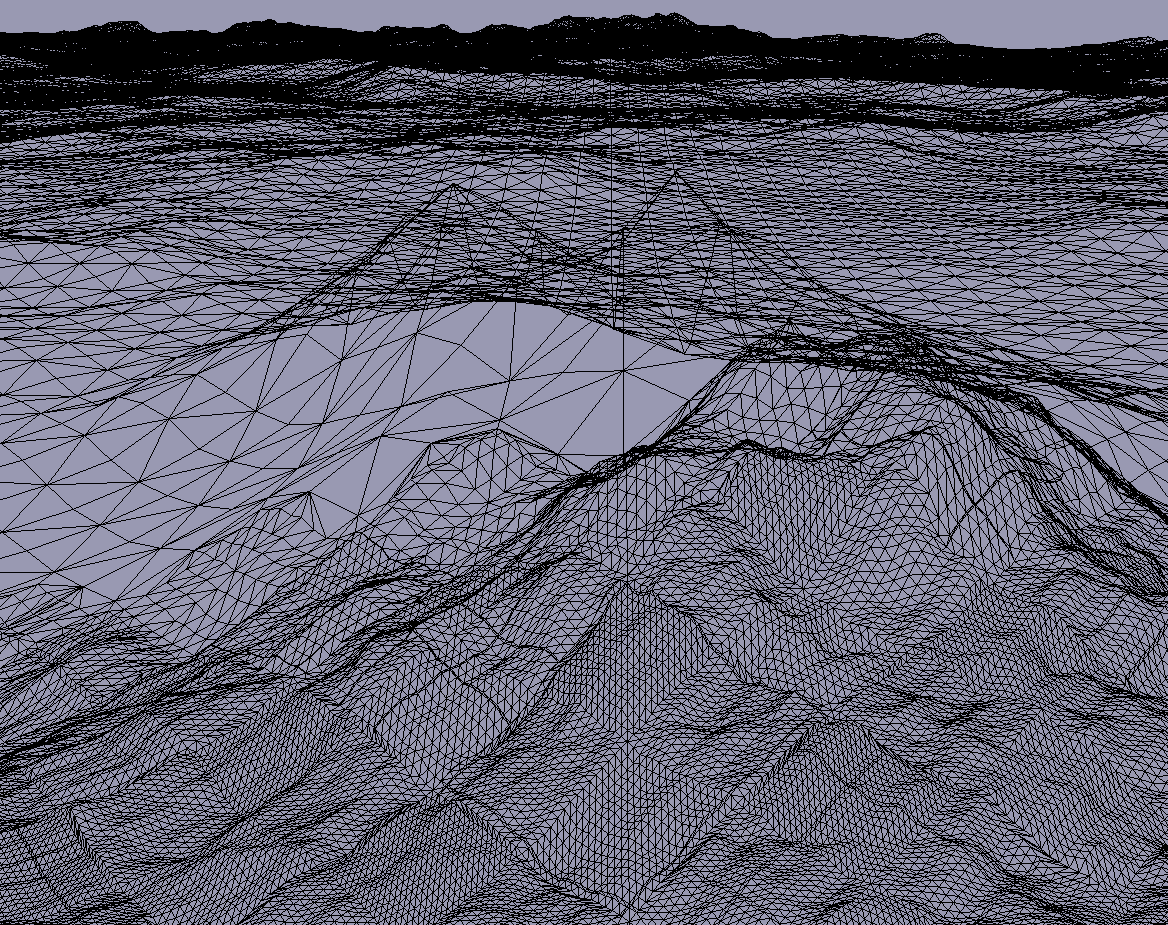
\includegraphics[width=0.75\textwidth]{img/cLOD.png}
	\caption{Different levels of detail for a chunk of terrain.}
	\label{fig:clod}
\end{figure}

In InfiniTerra, we use a chunk size of 1000x1000
units, with a resolution of 1600 vertices per chunk. One more advantage of chunking is that it
allows us to generate the terrain procedurally in chunks, which makes it easier to parallelize the
generation.

\section{Culling}
Culling is the process of determining which objects are visible to the camera and should be
rendered. One common technique used in culling is frustum culling, which involves checking if an
object is inside the camera's frustum before rendering it. This can greatly improve performance by
reducing the number of objects that need to be rendered.

\begin{figure}[H]
	\centering
	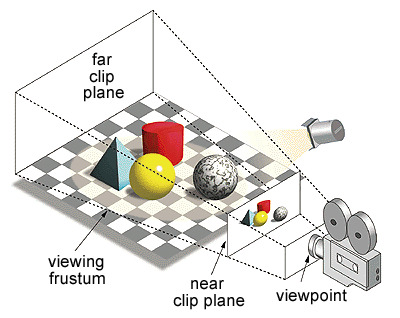
\includegraphics[width=0.75\textwidth]{img/frustum.jpg}
	\caption{The commonly used frustum culling technique.}
	\label{fig:frustum}
\end{figure}

In InfiniTerra, we use a simplified
culling technique to determine which chunks of terrain are visible to the camera and should be
rendered. This technique involves two steps:
\begin{itemize}
	\item \textbf{Distance-based culling:} Checking if the chunk is within a certain distance of the camera.
	\item \textbf{Direction-based culling:} Checking if the chunk is within the camera's field of view. 
	This is done with a simple dot product between the camera's forward vector and the vector from the camera to the chunk.
\end{itemize}


\section{Level of Detail (LOD)}

Level of Detail (LOD) is a technique used in computer graphics to optimize the rendering of complex
3D models by reducing the level of detail based on the distance from the camera. This allows the
rendering engine to display high-quality models when they are close to the camera and switch to
lower-quality models when they are far away. In InfiniTerra, we use an LOD system based on
tessellation to dynamically adjust the level of detail of the terrain based on the distance from
the camera. This is done by subdividing the terrain into smaller patches and increasing the level
of tessellation as the camera gets closer to the terrain. This affords us multi-resolution control
over every chunk of terrain, allowing the same mesh to be rendered with different levels of detail
depending on the distance from the camera.

\subsection{Tessellation}

Tessellation, a Vertex Processing stage in the OpenGL rendering pipeline, involves the subdivision 
of vertex data patches into smaller Primitives. This operation is controlled by two shader stages 
and one fixed-function stage. The tessellation process consists of three stages, forming an 
optional part of the Vertex Processing in the rendering pipeline. Two of these stages are 
programmable, with a fixed function stage in between. The Tessellation Control Shader (TCS) decides 
the degree of tessellation. Hence, the TCS primarily ensures continuity across patches. If two 
neighboring patches require different tessellation levels, the TCS invocations for these patches 
must use their tessellation controls to guarantee that the shared edge(s) between the patches have 
the same tessellation level. Without this safeguard, discontinuities can appear in what should be 
contiguous patches. The TCS is optional, and if not provided, default tessellation values can be 
used. The tessellation primitive generator subdivides the input patch based on the values computed 
by the TCS or provided as defaults. The Tessellation Evaluation Shader (TES) processes the 
tessellated patch and calculates the vertex values for each generated vertex.

\begin{figure}[H]
	\centering
	\begin{subfigure}[h]{0.45\textwidth}
		
\includegraphics[width=\textwidth]{img/triangle-patch.png}
		\caption{Caption for Figure 1}
		\label{fig:figure1}
	\end{subfigure}
	\hfill
	\begin{subfigure}[h]{0.45\textwidth}
		
\includegraphics[width=\textwidth]{img/quad-patch.png}
		\caption{Caption for Figure 2}
		\label{fig:figure2}
	\end{subfigure}
	\caption{Caption for the whole figure}
	\label{fig:both_figures}
\end{figure}

\section{Interface}
\label{ch:interface}
% User interface
InfiniTerra features a simple user interface that allows the player to control the camera and set
several parameters that affect the terrain generation. The user interface is implemented using the
ImGui library, which provides a simple and flexible way to create graphical user interfaces in
OpenGL applications. The interface features:
\begin{itemize}
	\item \textbf{FPS}: Displays the current frames per second.
	\item \textbf{Camera Position}: Displays the current position of the camera in the x, y, and z coordinates.
	\item \textbf{Capture Mouse}: Button to capture the mouse cursor. Pressing space will free the cursor.
	\item \textbf{Wireframe View}: Checkbox to enable or disable wireframe view of the terrain.
	\item \textbf{Terrain Height}: Slider to adjust the height of the terrain.
	\item \textbf{Min Tess Level}: Slider to adjust the minimum tessellation level of the terrain.
	\item \textbf{Max Tess Level}: Slider to adjust the maximum tessellation level of the terrain.
	\item \textbf{Min Tess Distance}: Slider to adjust the minimum tessellation distance of the terrain.
	\item \textbf{Max Tess Distance}: Slider to adjust the maximum tessellation distance of the terrain.
	\item \textbf{Fog Distance}: Slider to adjust the fog distance in the scene.
	\item \textbf{Grass Color}: Color picker to adjust the color of the grass in the terrain.
	\item \textbf{Dry Color}: Color picker to adjust the color of the dry areas in the terrain.
	\item \textbf{Snow Color}: Color picker to adjust the color of the snow in the terrain.
	\item \textbf{Sky Color}: Color picker to adjust the color of the sky.
	\item \textbf{Resolution}: Slider to adjust the resolution of the terrain.
	\item \textbf{Frequency}: Slider to adjust the frequency of the terrain.
	\item \textbf{Regenerate Terrain}: Button to regenerate the terrain with the current settings.
\end{itemize}

\begin{figure}[H]
	\centering
	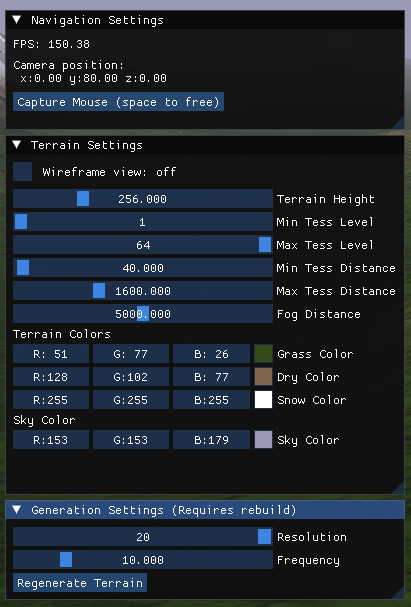
\includegraphics[width=0.75\textwidth]{img/interface.png}
	\caption{The user interface of InfiniTerra.}
	\label{fig:interface}
\end{figure}

\section{Performance}
\label{ch:performance}


InfiniTerra is capable of generating and rendering large terrains with high performance. The use of
compute shaders for terrain generation and tessellation for LOD allows the system to handle
hundreds of chunks of terrain with minimal impact on performance. The system runs at a stable XX
fps on a modern GPU, with the frame rate dropping slightly when the camera is close to the terrain
and the level of detail is high. The performance of the system can be further improved by
optimizing the terrain generation algorithm and the rendering pipeline. This could involve using
batched rendering to reduce the number of draw calls, optimizing the culling algorithm to reduce
the number of chunks that need to be rendered, and using more efficient data structures to store
the terrain data.

\subsection{System Specifications}
\label{ch:system-specs}

\begin{table}[H]
	\centering
	\begin{tabular}{|c|c|}
		\hline
		\textbf{Component} & \textbf{Specification}      \\
		\hline
		CPU                & 6-core Intel Core i7-10750H \\
		\hline
		GPU                & NVIDIA GeForce RTX 3060 Ti  \\
		\hline
		RAM                & 16 GB DDR4                  \\
		\hline
		Storage            & 1 TB SSD                    \\
		\hline
	\end{tabular}
	\caption{System Specifications}
	\label{tab:system-specs}
\end{table}

% Conclusion
\section{Conclusion}
\label{ch:conclusion}

The implementation of compute shaders, chunking, culling, and level of detail (LOD) techniques in
the terrain rendering system has significantly improved the performance and visual quality of
InfiniTerra. The use of compute shaders allows for efficient parallel computation on the GPU,
enabling tasks such as terrain generation and lighting calculations to be performed at high speeds.
Chunking and culling techniques ensure that only the visible chunks are rendered, reducing the
rendering workload and improving overall performance. The LOD system dynamically adjusts the level
of detail based on the distance from the camera, resulting in smooth transitions and optimized
rendering. These optimizations, combined with the user interface for controlling camera parameters
and terrain regeneration, provide a seamless and immersive experience for the player. Further
performance improvements can be achieved through optimization of the terrain generation algorithm
and rendering pipeline. By leveraging batched rendering, optimizing the culling algorithm, and
using efficient data structures, the system can handle even larger terrains with minimal impact on
performance. Overall, InfiniTerra demonstrates the power of compute shaders and advanced rendering
techniques in creating realistic and performant terrain systems.

% References
\bibliographystyle{plain}
\bibliography{references}

\end{document}